\begin{figure*}
    \label{fig:model}
    \centering
    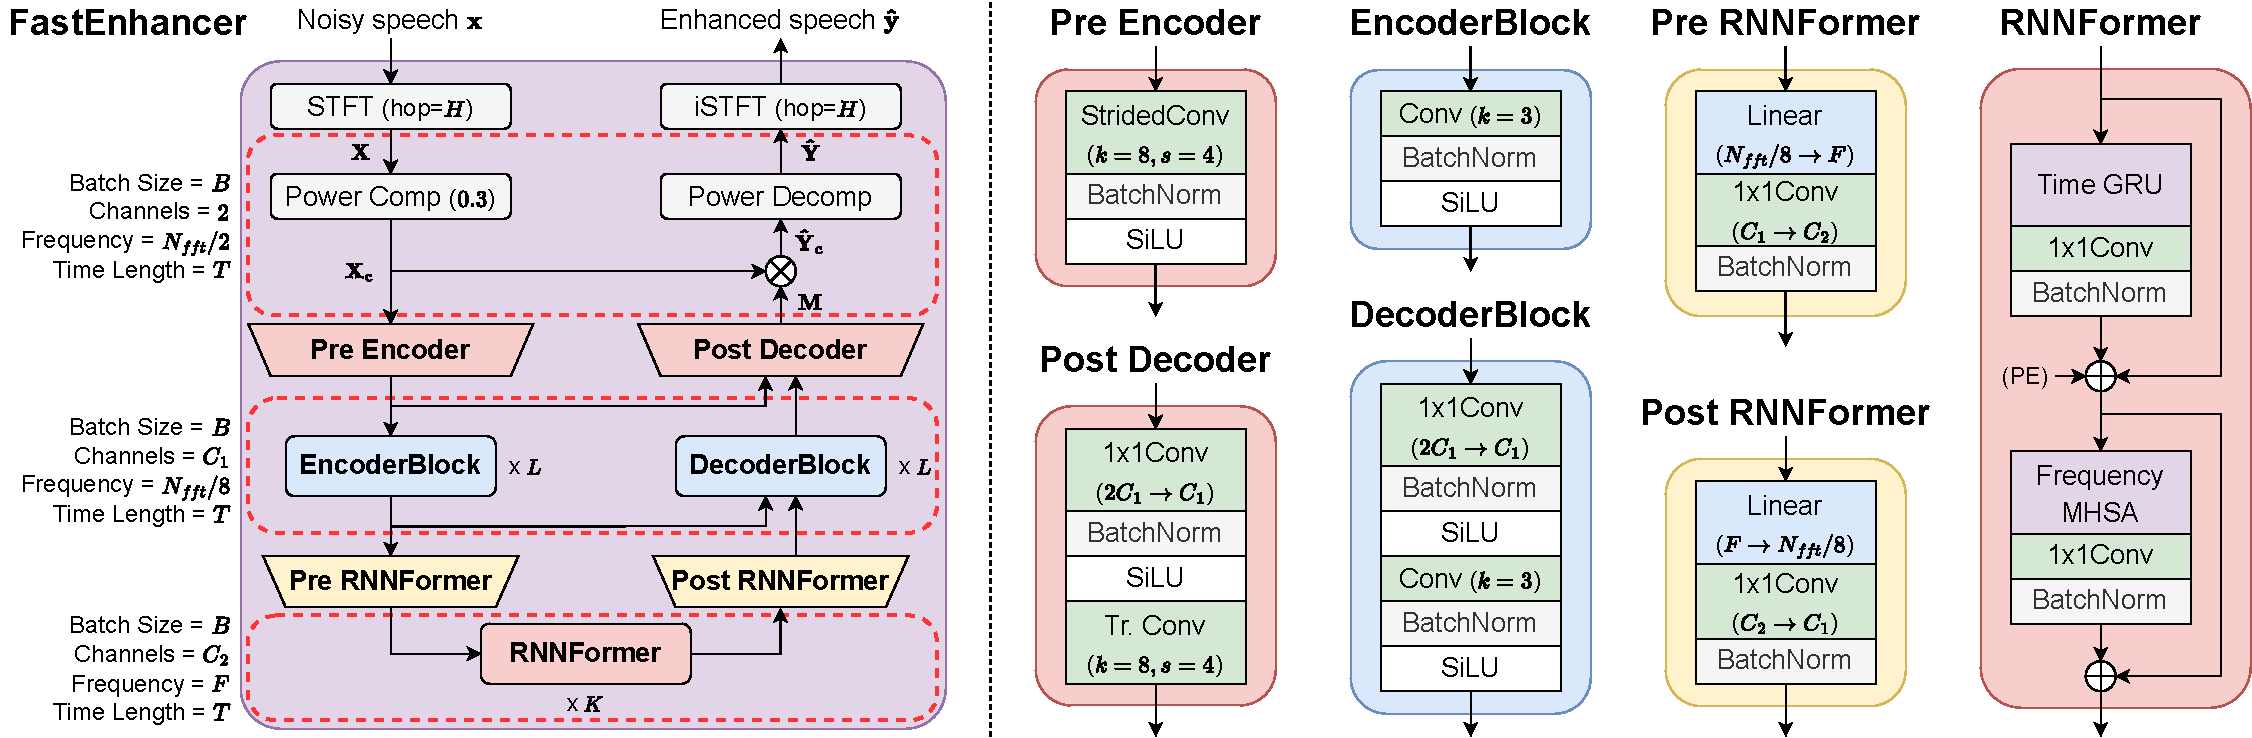
\includegraphics[width=1.0\linewidth]{fig_model.pdf}
    \vspace{-20pt}
    \caption{\textit{FastEnhancer} model architecture. Conv($k$), StridedConv($k$, $s$), and Tr. Conv($k$, $s$) denote a convolution, a strided convolution, and a transposed convolution respectively, with a kernel size of $k$ and a stride of $s$. 1x1Conv($A \rightarrow B$) represents a 1x1 convolution with $A$ input channels and $B$ output channels. Linear($A \rightarrow B$) represents a linear layer with $A$ input features and $B$ output features.}
    \vspace{-9pt}
\end{figure*}

This section details the architecture of \textit{FastEnhancer} as shown in Fig. \ref{fig:model}. We start by describing the input and output. We then present convolutional and normalization layers characterized by low latency for streaming inference. Finally, using those building blocks, we explain a simple encoder-decoder structure and our novel RNNFormer blocks. Note that we apply weight normalization \cite{weightnorm} and use the SiLU activation function \cite{silu} across the entire model.

\textbf{Input and Output} -- An input noisy speech $\textbf{x}$ is first transformed into a complex spectrogram $\textbf{X}=\text{STFT}(\textbf{x})$ with a Fourier transform size of $N_{fft}=512$ and a hop size of $H$. To mimic the dynamic compression nature of the human ear, we apply power compression as $\textbf{X}_c = |\textbf{X}|^c\cdot e^{j \angle \textbf{X}}$, where $c=0.3$. We then interpret $\mathbf{X}_c$ as a tensor with two channels (real and imaginary part) and $N_{fft}/2$ frequencies (for simplicity, we discard the highest frequency bin). Given $\mathbf{X}_c$, \textit{FastEnhancer} predicts a two-channel mask \textbf{M} and generates a power-compressed enhanced spectrogram $\hat{\textbf{Y}}_c=\textbf{M} \odot \textbf{X}_c$. After power decompression $\hat{\textbf{Y}} = |\hat{\textbf{Y}}_c|^{1/c}\cdot e^{j \angle \hat{\textbf{Y}}_c}$, the highest frequency bin is zero-padded and the final enhanced speech $\hat{\textbf{y}}=\text{iSTFT}(\hat{\textbf{Y}})$ is synthesized. $\hat{\textbf{y}}$ is then compared to a target clean speech $\textbf{y}$.

\textbf{Convolutional Layers} -- Causal convolutional layers with a time-axis kernel size greater than one introduce latency, because they require caching past frames to compute the current output frame. For a time-axis kernel size of $k$, a buffer of $k-1$ past frames is stored and concatenated with the current frame before the convolution operation. The latest $k-1$ frames are then stored in memory for the next computation. These memory operations significantly increase processing time (Section \ref{sec:ablation}). To ensure minimum latency, \textit{FastEnhancer} exclusively uses convolutions with a time-axis kernel size of one. Throughout this paper, all specified kernel sizes and strides for convolutions refer to the frequency axis.

\textbf{Normalization Layers} -- Speech enhancement models typically use either batch normalization (BN) \cite{batchnorm} or layer normalization (LN) \cite{layernorm}. While both methods introduce negligible number of parameters and MACs, BN can be converted into a simple multiplication-addition operation and fused into adjacent layers at inference time. In contrast, LN cannot be fused in the same manner, increasing the RTF (Section \ref{sec:ablation}). For this reason, we use BN layers throughout our model and fuse them into neighboring layers at inference time.

\textbf{Encoder and Decoder} -- The encoder starts with a pre-encoder network containing a strided convolution that reduces the frequency resolution from $N_{fft}/2$ to $N_{fft}/8$ while enlarging the channels from $2$ to $C_1$. It is followed by a stack of $L$ encoder blocks. The decoder contains $L$ decoder blocks, followed by a post-decoder network that restores the frequency resolution using a transposed convolution. Skip connections are used to link the encoder and decoder.

After the encoder blocks and before the decoder blocks, we append pre-RNNFormer and post-RNNFormer networks to bridge to the RNNFormer blocks. The pre-RNNFormer network is composed of a linear layer that reduces frequency resolution from $N_{fft}/8$ to $F$, followed by a convolution that reduces channels from $C_1$ to $C_2$. The post-RNNFormer network performs the reverse operations. The weight of the linear layer in pre-RNNFormer is initialized as a linear filterbank, and the weight of the linear layer in post-RNNFormer is initialized as a linear interpolation. We empirically found that training these weights offered no performance benefit over keeping them fixed. Therefore, we fixed those weights in all experiments.

\textbf{RNNFormer} -- \textit{FastEnhancer} contains $K$ RNNFormer blocks. Each block consists of two sub-blocks: a time-axis Gated Recurrent Unit (GRU) \cite{gru} block, and a frequency-axis Multi-Head Self-Attention (MHSA) \cite{transformer} block. This hybrid design is critical for low-latency and high-performance. For the time axis, a GRU is well-suited for streaming inference with minimal latency, whereas an MHSA requires a key-value caching that increases delay (as described in Section \ref{sec:related-dpn}). For the frequency axis, an MHSA is ideal as it can model global relationships and doesn't require caching.

The GRU block contains a sequence of a unidirectional GRU, a convolution, a BN layer, and a residual skip connection. The MHSA block follows an identical structure but replaces the GRU layer with an MHSA with four heads. We add a trainable positional encoding to the input of the first MHSA block.